\section{Evaluation}
\label{sec:evaluation}

  \subsection{Exhaustive search vs \atl orthogonal search}
  \label{sec:exhaustiveVSorthogonal}

  \begin{figure*}[tbhp]
    \centering
    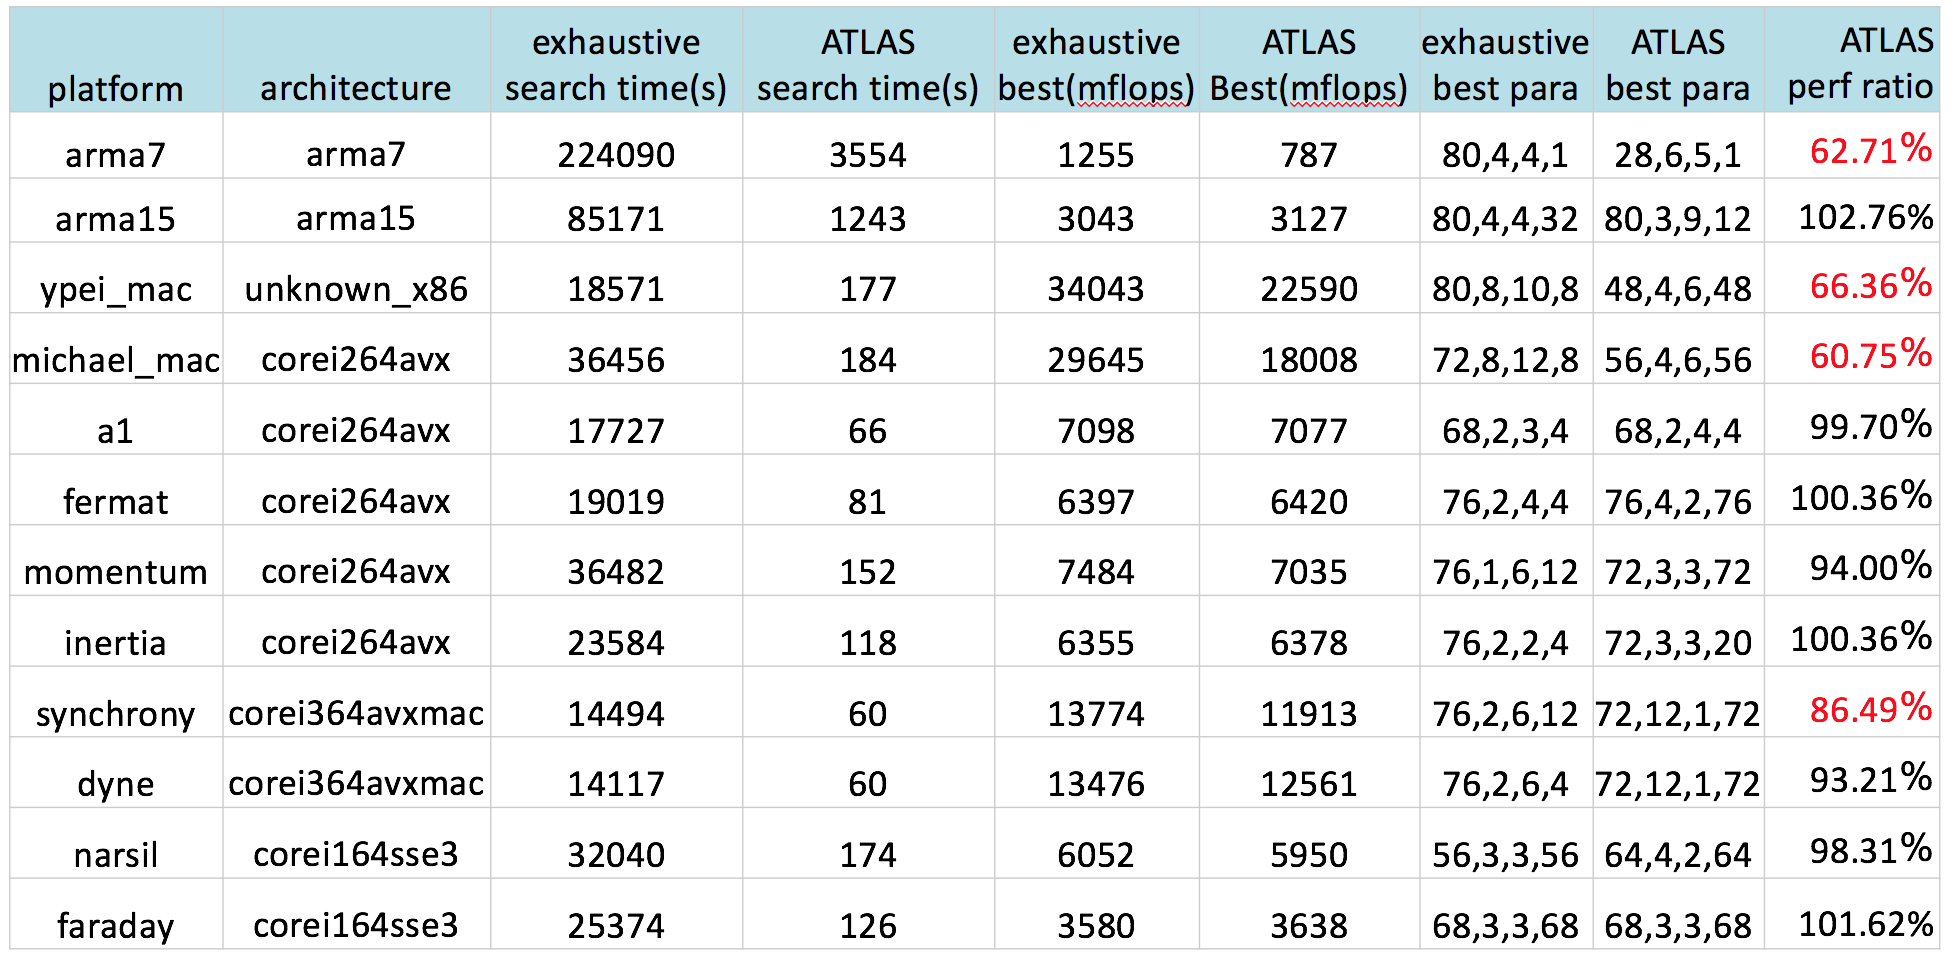
\includegraphics[width=0.9\textwidth]{images/exhaustiveVsorthogonal.png}
    \caption{Searching time comparison between exhaustive search and \atl orthogonal search}
    \label{fig:exhaustiveVsorthogonal}
  \end{figure*}

  \subsection{GEMM performance model}
  \label{sec:GEMMperf}

  \subsection{Capri-based ATLAS searching time}
  \label{sec:capri_atlas_searching}

  \begin{figure*}[tbhp]
    \centering
    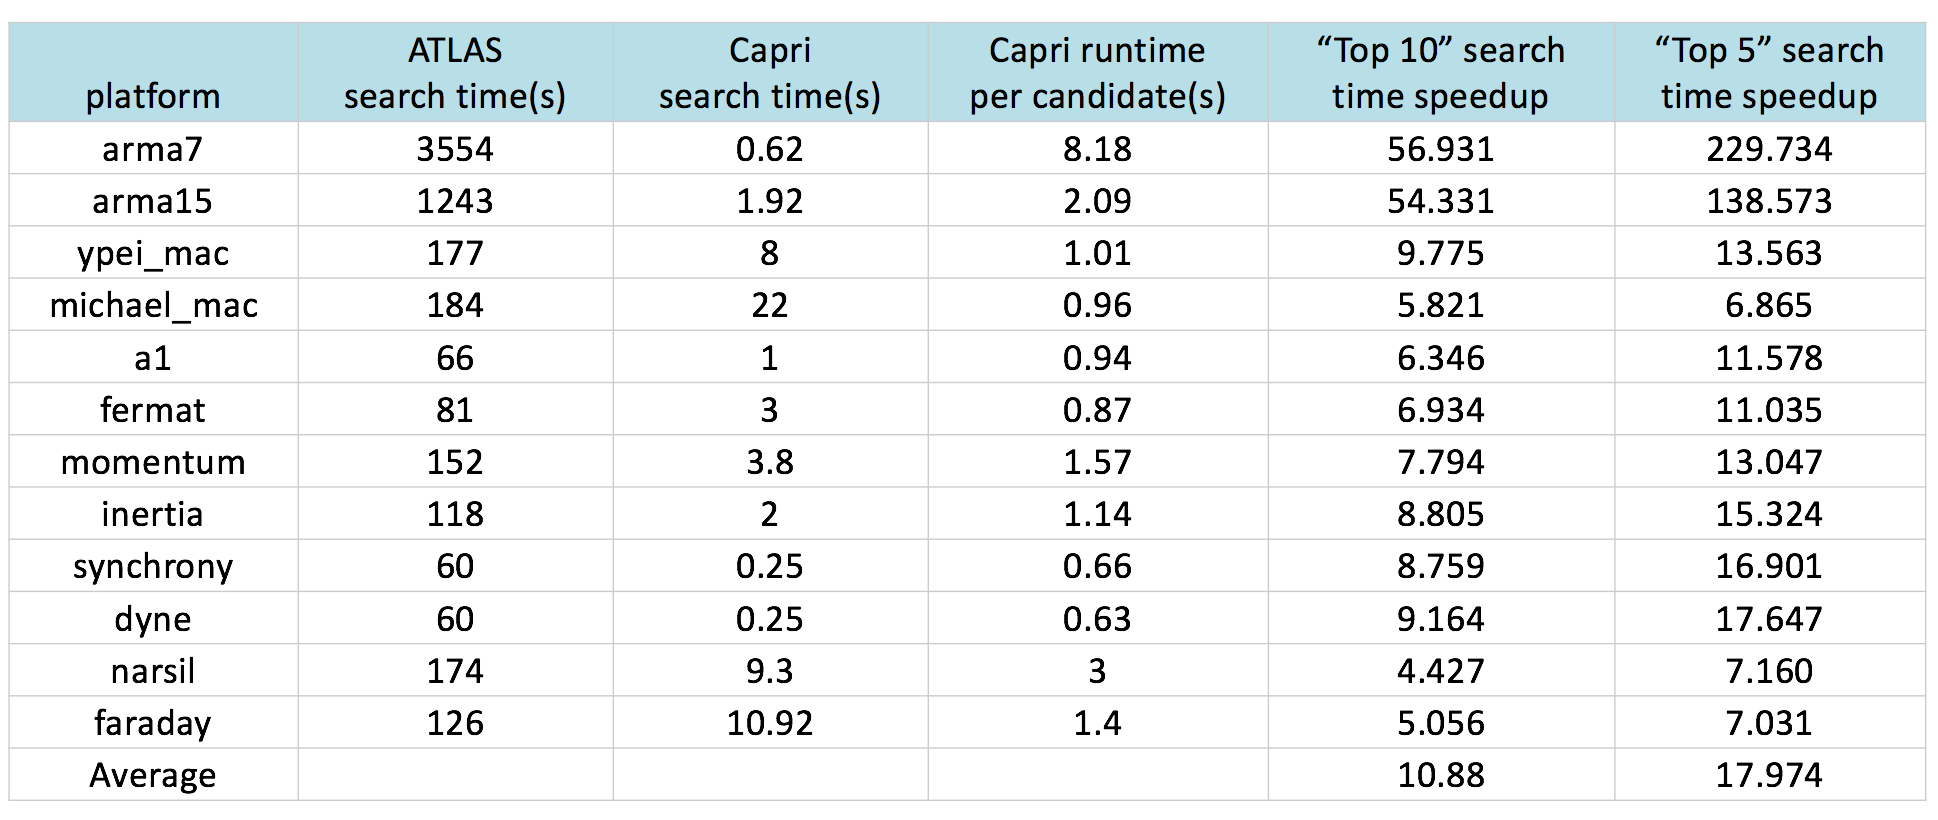
\includegraphics[width=0.9\textwidth]{images/timespeedup.png}
    \caption{Capri-based ATLAS searching time speedup}
    \label{fig:platforms}
  \end{figure*}

  \subsection{Capri-based ATLAS performance}
  \label{sec:capri_atlas_performance}

  \begin{figure*}[tbhp]
    \centering
    \begin{subfigure}[b]{1.0\linewidth}
      \centering
      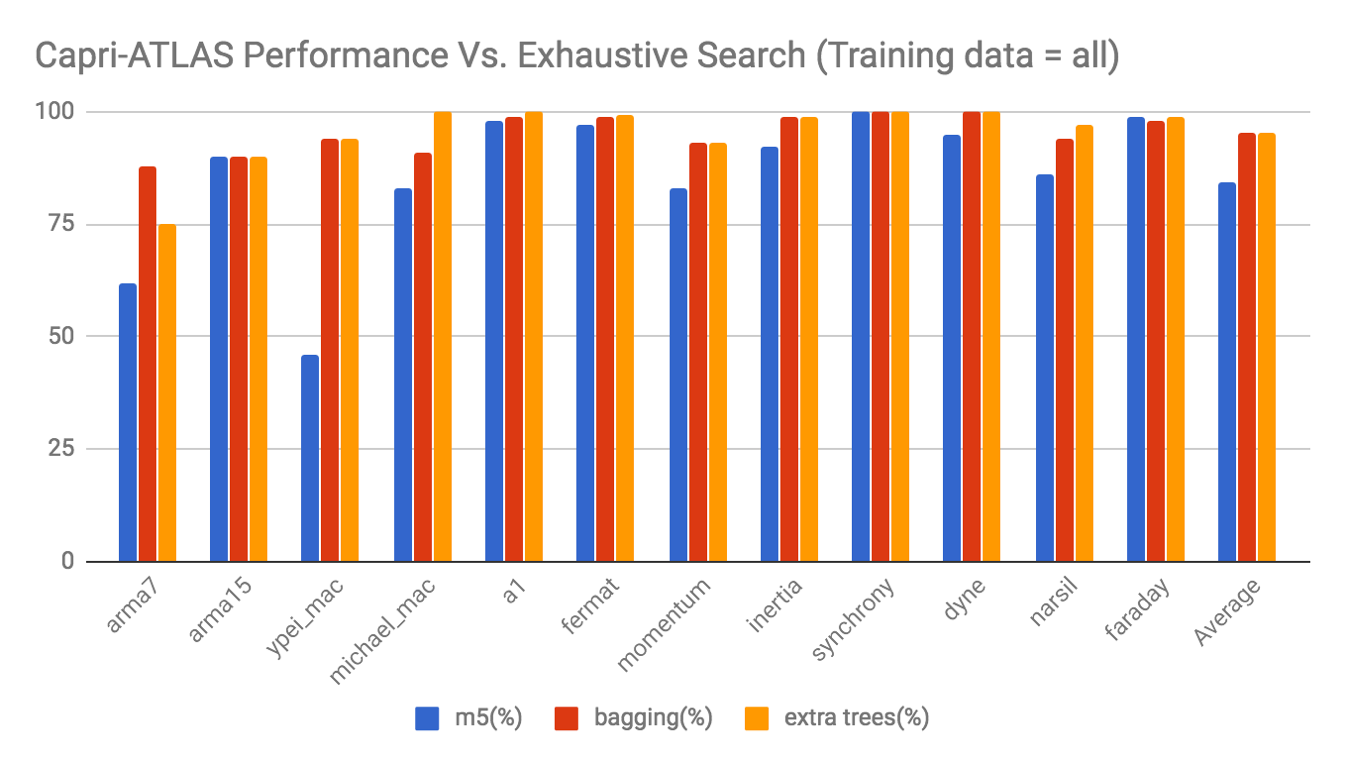
\includegraphics[width=0.85\textwidth]{images/all_perf.png}
      \caption{ }
      \label{fig:all_perf}
    \end{subfigure}
    \begin{subfigure}[b]{1.0\linewidth}
      \centering
      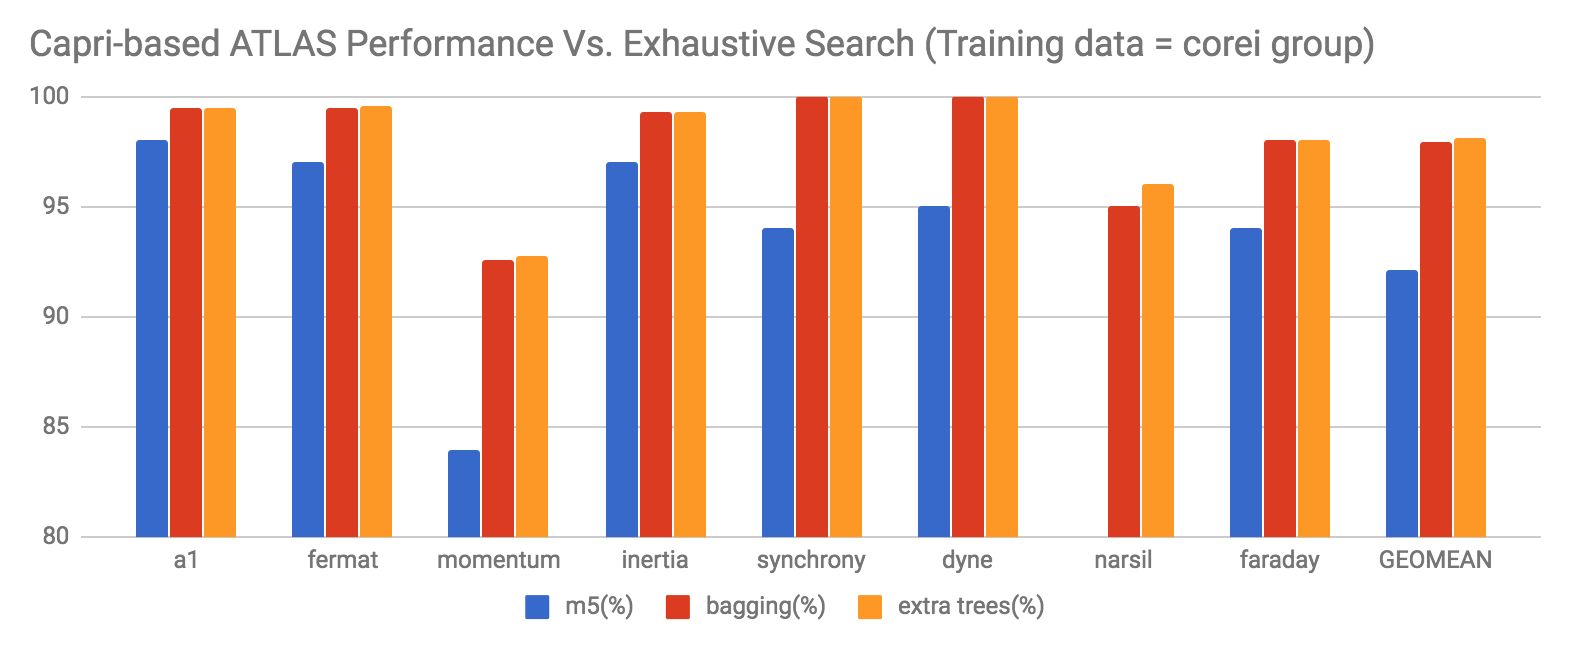
\includegraphics[width=0.85\textwidth]{images/corei_perf.png}
      \caption{ }
      \label{fig:corei_perf}
    \end{subfigure}
    \begin{subfigure}[b]{1.0\linewidth}
      \centering
      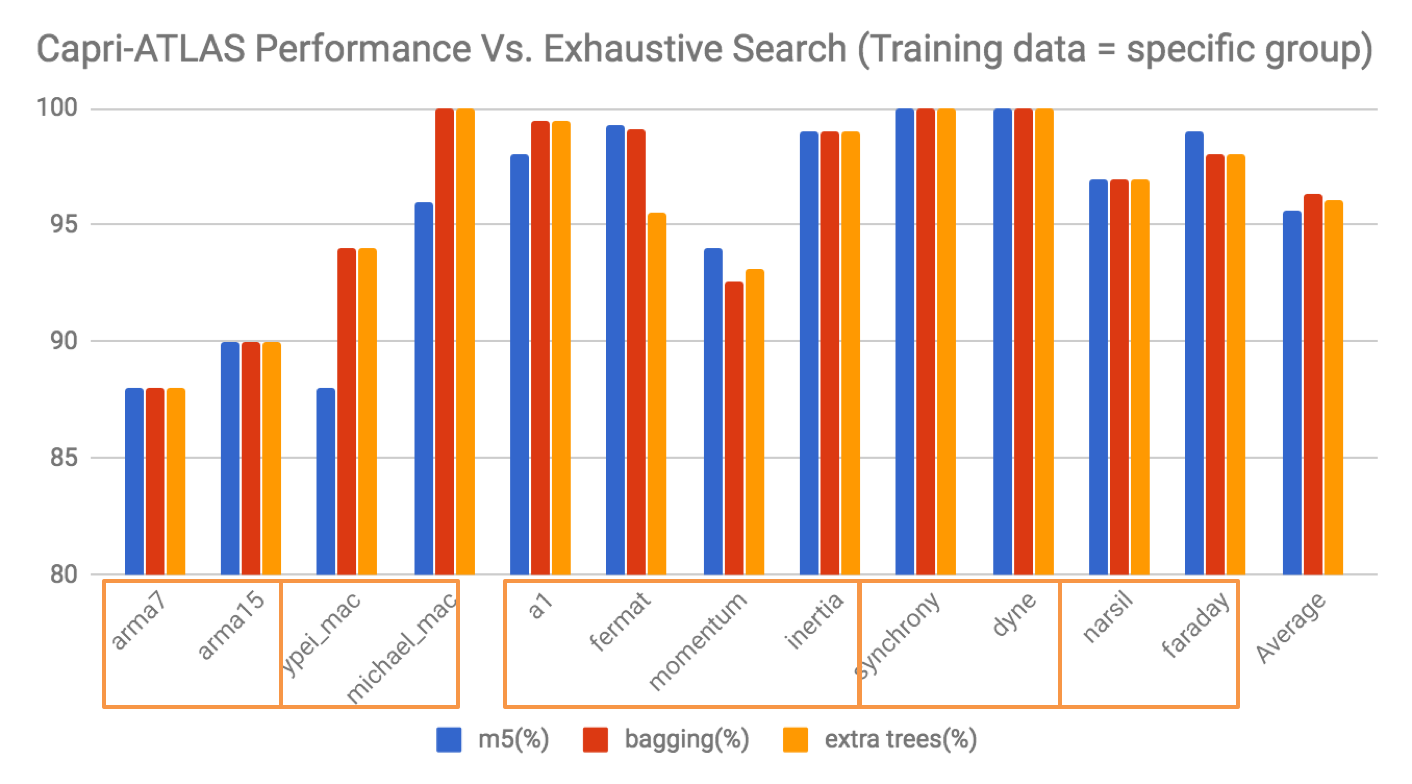
\includegraphics[width=0.85\textwidth]{images/specific_perf.png}
      \caption{ }
      \label{fig:specific_perf}
    \end{subfigure}
  \caption{Capri-based \atl Performance using different training sets}
  \end{figure*}

  \subsection{Parameter sensitivity}
  \label{sec:parametersensitivity}

    \subsubsection{Training set}
    \label{sec:training_set}

    \subsubsection{Top M constraint}
    \label{sec:top_m}
